\section{Datenstrukturen}
\label{datastructures}

Zur Beschleunigung von atomistischen Simulationen mit Parsivald finden effiziente Algorithmen zur Suche und Manipulation von Atomen auf Basis verschiedener Datenstrukturen Anwendung, welche im Folgenden zwecks der Beschreibung von Atompositionen in teilperiodischen Simulationsräumen für Off-Lattice-KMC-Simulationen untersucht werden sollen.
Gegenüber optimalen Algorithmen für allgemeine Probleme, wie sie in verfügbarer Software genutzt werden, ermöglicht die genaue Modell- und Systemkenntnis die Abwägung der Häufigkeit von Operationen gegen deren Laufzeiten,
wodurch die Wahl der optimalen Datenstruktur zur Maximierung von Größe, Genauigkeit und Geschwindigkeit von Off-Lattice-KMC-Simulationen von Gasphasenabscheidungen ermöglicht wird.

\subsection{Numerische Voraussetzungen an Gasphasenabscheidungen}

Für eine effiziente KMC-Simulation werden für zu untersuchende Gasphasenabscheidungen folgende Voraussetzungen getroffen:
Zuerst sollten die KMC-Ereignisse \textbf{lokal}, also auf eine geringe Reichweite begrenzt sein.
Das bedeutet auch, dass die Atome über \textbf{niedrige Diffusionskoeffizienten} verfügen, was sich aus der Notwendigkeit ergibt, im statischen Gleichgewicht befindliche Bereiche des Simulationsraumes von atomistischen Simulationen auszuschließen.
Weiterhin werden \textbf{scharfe Phasengrenzen} vorausgesetzt, also zweidimensionale Grenzflächen, die sich durch eine vergleichsweise geringe Menge von Atomen darstellen lassen.
Zuletzt finden die Simulationen aus praktischen Gründen in \textbf{teilperiodischen Räumen} statt, also Räumen, die in der xy-Ebene periodisch, aber in z-Richtung beliebig ausgedehnt sein können.

%% Daraus ergeben sich jeweils Vor- und Nachteile für verschiedene Datenstrukturen, so dass etwa für die Vereinigung zweier disjunkter Triangulation (Stitching) in periodischen Räumen zusätzlicher Aufwand gegenüber nichtperiodischen Räumen betrieben werden muss.
%% Die größten Vorteile ergeben sich aus der Lokalität von Ereignissen, da so für die meisten Datenstrukturen nur kleine Teilstrukturen überprüft und aktualisiert werden müssen.

\subsection{Vergleich der Laufzeiten mit verschiedenen Datenstrukturen}

Als Datenstrukturen stehen \textbf{Atomlisten}, \textbf{Nachbarschaftslisten} (NB-Listen), lineares \textbf{Binning}, Binning in \textbf{Octrees}, \textbf{k-d-Bäume} und \textbf{Delaunay-Triangulationen} zur Auswahl, von denen eine Auswahl in Abbildung~\ref{fig:datastructures} dargestellt ist.
In Anhang~\ref{appendix_dataoverview} werden diese knapp vorgestellt, wobei auf die drei zuletzt genannten in den folgenden Abschnitten näher eingegangen wird.

Atomistische KMC-Simulationen beschränken sich auf die Manipulations-Operationen zur \textbf{Einfügung}, \textbf{Modifikation} und \textbf{Entfernung} von Atomen, \textbf{Konstruktion} der Datenstruktur sowie auf die Suchoperationen der \textbf{Nachbarschaftssuche}, \textbf{Bereichssuche} und \textbf{Oberflächensuche}, die jeweils im Anhang in Tabelle~\ref{tab:dataops} kurz beschrieben werden.
Die Effizienz dieser Operationen geht dabei aus deren asymptotischer Laufzeit hervor, welche üblicherweise in asymptotischer Notation (\BigO{}) angegeben wird.

Bei KMC-Simulationen überwiegen die drei Suchoperationen, da sie für jedes Ereignis beim Aufbau der KMC-Ereignislisten durchgeführt werden müssen, wo hingegen die Manipulationen nur für das tatsächlich durchgeführte Ereignis ausgeführt werden müssen.
Somit liegt das Auswahlkriterium der Datenstruktur bei der Effizienz ihrer Suchoperationen, mit Ausnahme der Nachbarschaftslisten und k-d-Bäume, deren Manipulationsoperationen für große Simulationsräume \todo{phrasing}zu langsam sind.
Die Ergebnisse der Laufzeit-Analysen der sieben Operationen auf den vorgestellten Datenstrukturen werden in Tabelle~\ref{tab:dataruntimes} zusammen gefasst, wofür Tabelle~\ref{tab:datasymbols} die verwendeten Symbole erklärt.

%% \begin{figure}[h]
%%   \captionsetup[subfigure]{singlelinecheck=false}{
%%     \def\subfigwidth{0.23\textwidth}
%%     \def\svgwidth{\textwidth}
%%     \begin{subfigure}[t]{\subfigwidth}
%%       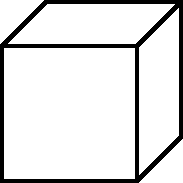
\includegraphics[width=\textwidth]{datastructures-a}
%%       \subcaption{Listen}
%%     \end{subfigure}
%%     \hfill
%%     \begin{subfigure}[t]{\subfigwidth}
%%       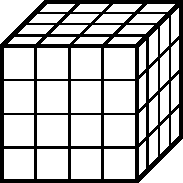
\includegraphics[width=\textwidth]{datastructures-b}
%%       \subcaption{Binning}
%%     \end{subfigure}
%%     \hfill
%%     \begin{subfigure}[t]{\subfigwidth}
%%       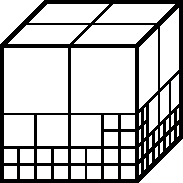
\includegraphics[width=\textwidth]{datastructures-c}
%%       \subcaption{Octree}
%%     \end{subfigure}
%%     \hfill
%%     \begin{subfigure}[t]{\subfigwidth}
%%       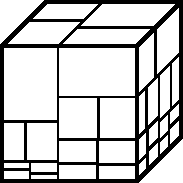
\includegraphics[width=\textwidth]{datastructures-d}
%%       \subcaption{k-d-Baum}
%%     \end{subfigure}
%%   }
%%   \caption[Übersicht über Partitionen des Simulationsraumes]{
%%     Übersicht über Partitionen des Simulationsraumes für einige Datenstrukturen.
%%     k-d-Baum-Partitionen sind dynamisch und ändern sich mit jeder Manipulation.
%%   }
%%   \todo[inline]{Hinweis von Jörg: Bild weglassen.}
%%   \label{fig:datastructures}
%% \end{figure}


\begin{table}[h]
  \centering

  \caption{Abschätzung der Komplexität für verschiedene Datenstrukturen und Operationen}
  \label{tab:dataruntimes}
  \begin{tabularx}{\textwidth}{|X|*8c|}
    \hline
    \textbf{Datenstr.} & Konstr.         & Einfüg.         & Modif.          & Entf.           & Ortss.                     & NB-Su.              & Oberfl.        & RAM                         \\
    \hline
    Atomlisten         & \cG{$n$}        & \cG{$1$}        & \cG{$1$}        & \cG{$1$}        & \cR{$n$}                   & \cR{$n$}            & \cR{$n$}       & \cG{$n$}                    \\
    NB-Listen          & \cY{$n\log{n}$} & \cR{$n$}        & \cR{$n$}        & \cR{$n$}        & \cR{$n$}                   & \cG{$1$}            & \cR{$n$}       & \cR{$\frac{r_c^3}{s^3}n^2$} \\
    Binning            & \cG{$n$}        & \cG{$1$}        & \cG{$1$}        & \cG{$1$}        & \cG{$r_s^3$}               & \cG{$r_s^3$}        & \cR{$c$}       & \cY{$n+c$}                  \\
    Octree             & \cY{$n\log{c}$} & \cY{$\log{c}$}  & \cY{$\log{c}$}  & \cG{$1$}        & \cY{$r_s^3\log{c}$}        & \cY{$r_s^3\log{c}$} & \cY{$\log{c}$} & \cY{$n+c^\frac{2}{3}$}      \\
    k-d-Baum           & \cY{$n\log{n}$} & \cY{$\log{n}$}  & \cY{$\log{n}$}  & \cY{$\log{n}$}  & \cY{$r_s^3\log{n}$}        & \cY{$r_s^3\log{n}$} & \cY{$\log{n}$} & \cG{$n$}                    \\
    Delaunay           & \cY{$n\log{n}$} & \cY{$k\log{k}$} & \cY{$k\log{k}$} & \cY{$k\log{k}$} & \cG{$r_s^3+n^\frac{1}{3}$} & \cG{$r_s^3$}        & \cG{$1$}       & \cY{$nk$}                   \\
    \hline
    %Atomfeld          & \cG{$n$}        & \cG{$1$}        & \cG{$1$}        & \cG{$1$}        & \cR{$n$}                   & \cR{$n$}            & \cR{$n$}       & \cG{$n$}                    \\
  \end{tabularx}
  \vspace{1em}
  \hspace{0.15\textwidth}
  \begin{tabularx}{0.6\textwidth}{|C|C|C|}
    \hline
    \cG{optimal} & \cY{vertretbar} & \cR{ineffizient} \\
    \hline
  \end{tabularx}

  \vspace{1em}

  \oddrowcolors
  \caption{Symbole für Laufzeit- und Speicherabschätzungen}
  \label{tab:datasymbols}
  \begin{tabularx}{\textwidth}{|cX|cX|}
    \hline
    \textbf{Symbol} & \textbf{Bedeutung}                 & \textbf{Symbol} & \textbf{Bedeutung} \\
    \hline
    \BigO{}         & Worst-Case-Komplexität             & $n$             & Zahl der Atome     \\
    $k$             & Zahl von Nächstnachbarn            & $b$             & Zahl der Bins      \\
    $k_r$           & Zahl von Nachbarn mit $d \leq r_c$ & $r_c$           & Cutoff-Radius      \\
    $r_s$           & Suchradius                         & $s$             & lineare Raumgröße  \\
    \hline
  \end{tabularx}

\end{table}

\clearpage
\subsection{Effiziente Datenstrukturen}

Beim Vergleich der Datenstrukturen in Tabelle~\ref{tab:dataruntimes} stellen sich Octrees, k-d-Bäume und Delaunay-Triangulationen als Favoriten für Off-Lattice KMC-Simulationen heraus, die in den folgenden Abschnitten kurz eingehender vorgestellt und diskutiert werden sollen.
Der Speicherverbrauch der untersuchten Datenstrukturen ist praktisch linear und wird deshalb nicht als Auswahlkriterium zu Rate gezogen.
Wie Untersuchungen an Simulationsräumen verschiedener Größe zeigen, wird erst für \num{1.9e9} Atome die Grenze des Hauptspeichers erreicht (Abschnitt~\ref{goldscalability}).

\subsubsection{Octrees}
\label{dataoctree}

Octrees sind eine Optimierung raumfüllender orthogonaler Partitionierungen, wie sie üblicherweise für Binning-Methoden genutzt werden, bei der statt linearer Adressierung auf einen mehrdimensionalen Binärbaum zurück gegriffen wird, woher auch der Name stammt (1D: Binary Tree, 2D: Quadtree, 3D: Octree, etc.).
Der Simulationsraum wird rekursiv in jeweils 8 disjunkte geometrisch ähnliche Unterzellen halber Breite aufgeteilt, wodurch die eigentlichen Bins in der festen Tiefe $\frac{\log{c}}{d\log{2}}$ liegen.

Damit steigt die Adressierungszeit für einzelne Zellen auf \BigO{\log{c}}, doch werden nur die Bins allokiert, die tatsächlich gefüllt sind (Abbildung~\ref{fig:octree}), wodurch leere Superzellen bei Suchoperationen automatisch übergangen werden.
Als Resultat sind für Oberflächensysteme der Speicherbedarf und die Laufzeit von Suchoperationen eines dreidimensionalen Simulationsraumes auf die eines zweidimensionalen Systemes reduziert.
Theoretisch sind mit Access Caching, Bitweiser Adressierung, Surface Flagging oder Height Mapping noch weitere Anpassungen möglich, allerdings verbessert sich dabei nur der Laufzeitfaktor, nicht die asymptotische Laufzeit, weshalb sie nur am Rand genannt sein sollen.

%% \begin{algorithm}
%%   \begin{algorithmic}
%% %    \Input $atoms$ - Liste der Atome
%% %    \Input $size[3]$ - Größe des Simulationsraumes
%% %    \Input $depth$ - Tiefe des Octrees (Legt die Zellgröße fest)
%% %    \Assumption Alle Atome befinden sich im Simulationsraum
%% %    \Result Stammzelle eines Octrees, der alle Atome enthält
%%     \State
%%     \Function{construct-octree}{$atoms, spacesize, depth$}
%%     \State $cellsize[0] \gets spacesize[0]\cdot2^{-depth}$
%%     \State $cellsize[1] \gets spacesize[1]\cdot2^{-depth}$
%%     \State $cellsize[2] \gets spacesize[2]\cdot2^{-depth}$
%%     \State $root \gets$ new Octree($depth$)
%%     \ForAll{$atom$ in $atoms$}
%%     \State $cellindex[0] \gets \lfloor atom.pos[0] / cellsize[0] \rfloor$
%%     \State $cellindex[1] \gets \lfloor atom.pos[1] / cellsize[1] \rfloor$
%%     \State $cellindex[2] \gets \lfloor atom.pos[2] / cellsize[2] \rfloor$
%%     \State $cell \gets$ \Call{getcell-octree}{$root, cellindex$, true}
%%     \State \Call{add-atom}{cell, atom}
%%     \EndFor
%%     \State \Return $root$
%%     \EndFunction
%%   \end{algorithmic}
%%   \caption[Octree-Konstruktion]{Octree-Konstruktion: Es handelt sich um einen typischen Binning-Algorithmus, dessen Octree-Eigenschaften in der Funktion \Call{getcell-octree}{} liegen.}
%%   \label{alco:octree-construction}
%% \end{algorithm}

\begin{figure}
  \centering
  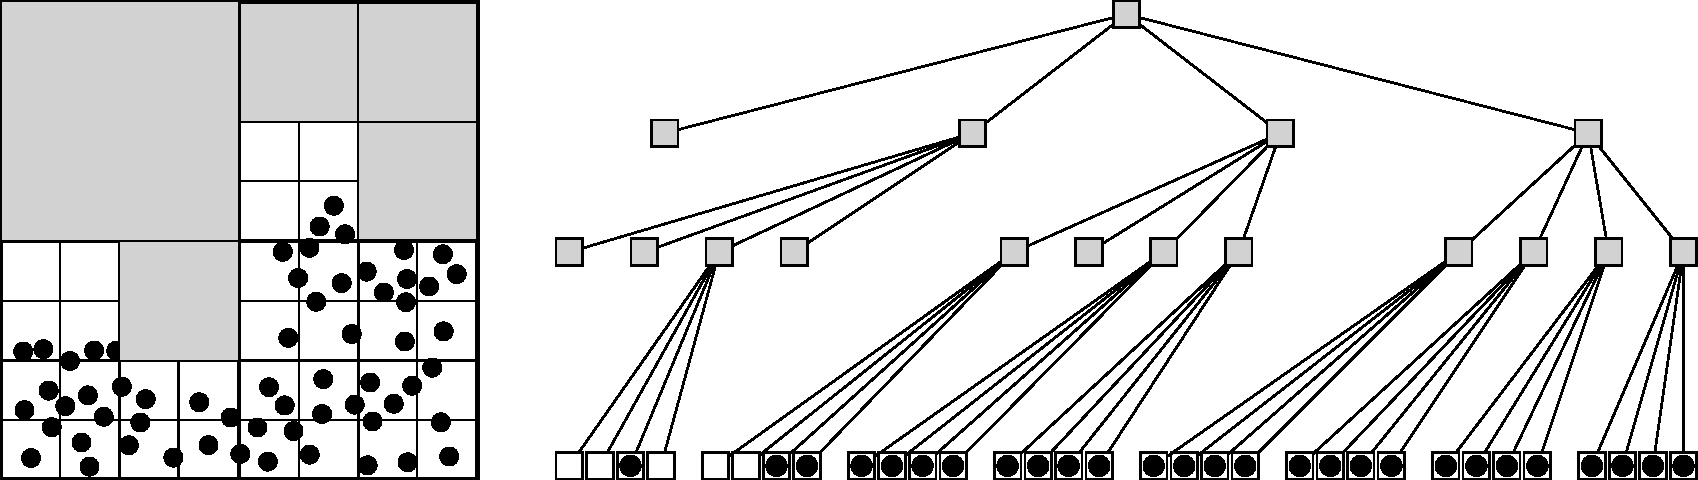
\includegraphics[width=\textwidth]{octree}
  \caption[Veranschaulichung der Funktionsweise eines Octrees]{
    Quadtree zur Veranschaulichung der Funktionsweise eines Octrees:\\
    Räumliche Unterteilung eines Raumes mit zugehörigem Baum von Zellen.
  }
  \label{fig:octree}
\end{figure}

%% \begin{algorithm}
%%   \begin{algorithmic}
%%     %    \Input $root$ - Stammzelle des Octrees
%%     %    \Input $i[3]$ - globale Adresse der Zielzelle
%%     %    \Input $allocate$ - Ob die Zelle neu erstellt werden soll
%%     \Result null falls leer, sonst Zielzelle
%%     \State
%%     \Function{getcell-octree}{$cell, id, allocate$}
%%     \State $d \gets $\Call{depth}{root}
%%     \Comment{Relative Tiefe, an der sich die Zielzellen befinden}
%%     \If{$d = 0$}
%%     \State\Return cell
%%     \EndIf
%%     \If{not $cell.children$}
%%     \If{allocate}
%%     \State $cell.children \gets $new cell[8]
%%     \Else
%%     \State \Return null
%%     \EndIf
%%     \EndIf
%%     \State $childid \gets $\Call{bitand}{id[0], $2^{d-1}$}
%%     + $2\cdot$\Call{bitand}{id[1], $2^{d-1}$}
%%     + $4\cdot$\Call{bitand}{id[2], $2^{d-1}$}
%%     %    \State \Comment{Indiziert die Subzelle aus der globalen Position}
%%     \State \Return\Call{getcell-octree}{$cell.children[childid], i, allocate$}
%%     \EndFunction
%%   \end{algorithmic}
%%   \caption[Zell-Adressierung in Octrees]{Rekursive Zell-Adressierung und -Allokierung im Octree: Bei jedem Schritt wird das Problem in 8 Unterzellen geteilt, woraus eine Laufzeit von \BigO{d}$=$\BigO{\log{c}} resultiert}
%%   \label{algo:octreeaddressing}
%% \end{algorithm}

\subsection{k-d-Bäume}
\label{datakdtree}

Für Nachbarschafts- und Bereichssuchen wird wegen ihrer hervorragenden Sucheffizienz oft auf k-d-Bäume zurückgegriffen, die einen kartesischen Raum in orthogonale Zellen mit jeweils einem Atom unterteilen, wodurch sich ein balancierter Binärbaum ergibt, an dessen Knoten die Atome liegen.
Durch implizite Betrachtung von Abstandsrelationen bei der Konstruktion (Abbildung~\ref{fig:kdtree}) lassen sich Abstands- oder Bereichssuchen in \BigO{\log{n}} durchführen, während Nachbarschaftssuchen von $N$ Atomen in Kombination mit einem Heap in \BigO{\log{n}\log{N}} möglich sind.

Nachteile ergeben sich bei Modifikationen von Atomen, die durch Baumrotation in \BigO{\log{n}} aufgelöst werden müssen und im schlimmsten Fall den gesamten Baum neu strukturieren.
Durch die einseitige, dichte und gleichverteilte Hinzufügung von Atomen während einer Oberflächenabscheidung ist dieser Fall allerdings wahrscheinlich, da der Baum auch für große Mengen von Atomen regelmäßig in z-Richtung aus der Balance gebracht wird.
Deshalb bieten sich k-d-Bäume zwar für allgemeine Suchoperationen in Off-Lattice-Strukturen an, sind aber nicht für effiziente KMC-Simulationen geeignet.

\begin{figure}
  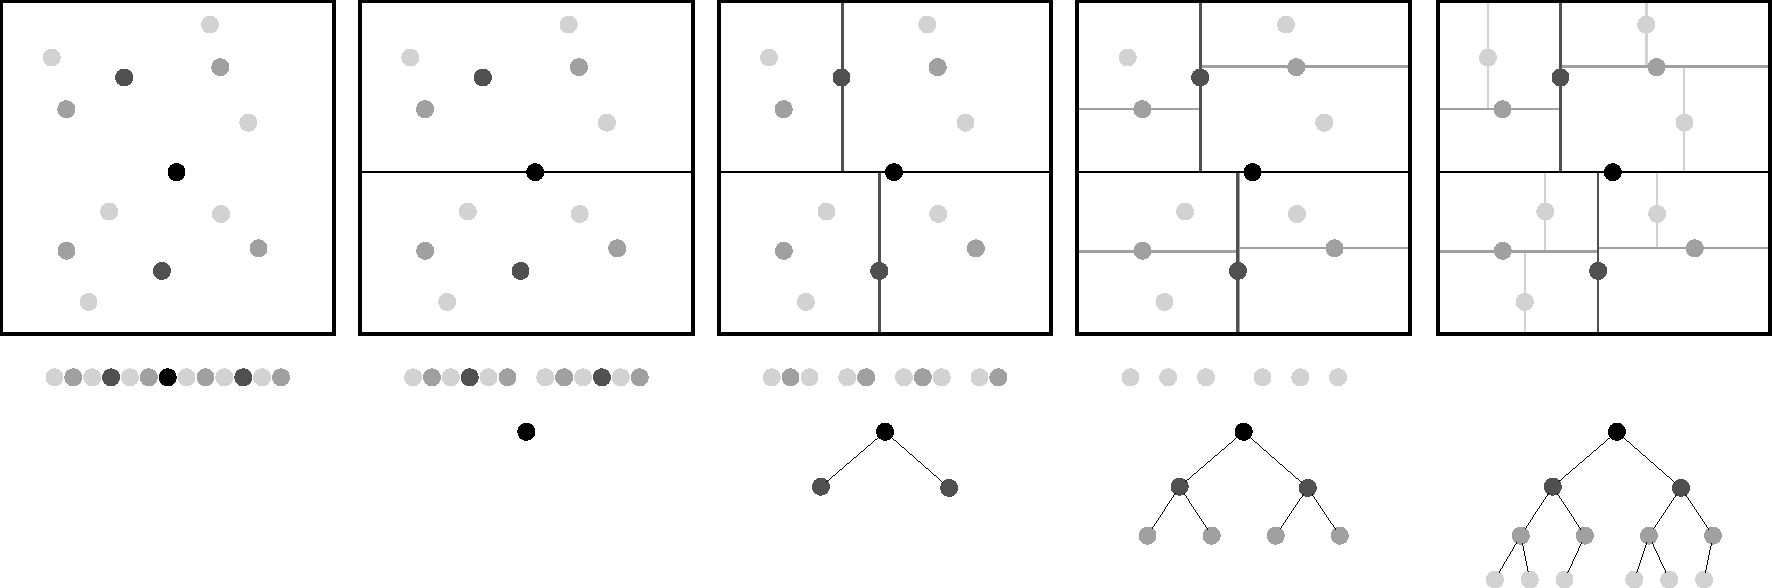
\includegraphics[width=\textwidth]{kdtree-tree}
  \caption[Konstruktion eines k-d-Baumes]{
    Konstruktion eines k-d-Baumes:
    Der Median der sortierten Punkte wird zur Wurzel des Baumes; die beiden Teilmengen rekursiv zu k-d-Bäumen
  }
  \label{fig:kdtree}
\end{figure}

%% \begin{algorithm}
%%   \begin{algorithmic}
%%     \Input $points$ - Liste von Punkten
%%     \Input $k$ - Dimensionalität des Simulationsraumes
%%     \Result Root-Element eines vollständigen KD-Baumes aus diesen Punkten
%%     \State
%%     \Function{construct-kdtree}{$points, dim\gets0$}
%%     \State $n\gets$\Call{length}{points}
%%     \If{$n=0$}
%%     \State \Return null
%%     \Else
%%     \State \Call{sort}{$points, dim$} \Comment{Sortiert $points$ nach pos[$dim$]}
%%     \State $root\gets{}points\left[\lfloor\frac{n}{2}\rfloor\right]$
%%     \State $dim\gets(dim+1)\mod{k}$
%%     \State $root.left \gets$ \Call{construct-kdtree}{$points\left[0:\lfloor\frac{n}{2}\rfloor-1\right], dim$}
%%     \State $root.right \gets$ \Call{construct-kdtree}{$points\left[\lfloor\frac{n}{2}\rfloor+1:n-1\right], dim$}
%%     \State \Return $root$
%%     \EndIf
%%     \EndFunction
%%   \end{algorithmic}
%%   \caption[Konstruktion eines k-d-Baumes]{Rekursive Konstruktion eines k-d-Baumes (naive Implementierung)}
%%   \label{algo:kdtree-construction}
%% \end{algorithm}

\subsection{Delaunay-Triangulation}
\label{datadelaunay}

\begin{figure}
  \centering
  \def\svgwidth{\textwidth}
  \input{img/delaunay.pdf_tex}
  \caption[Beispiel des Delaunay-Kriteriums]{
    In der Delaunay-Triangulation (c) einer Punktwolke (a) dürfen sich keine weiteren Punkte im Umkreis jedes Simplexes (b) befinden
  }
  \label{fig:delaunay}
\end{figure}

Eine dritte Partitionsmethode findet sich in der Delaunay-Triangulation\todo{Ref?}, welche jedoch asymmetrisch und nicht-orthogonal arbeitet, indem die konvexe Hülle der Punktwolke raumfüllend in disjunkte k-dimensionale Simplexe\footnote{Ein $k$-Simplex ist ein Objekt in $k$ Dimensionen mit $k+1$ Eckpunkten, die untereinander mit geraden Kanten verbunden sind. Somit ist ein 1-Simplex eine Linie, ein 2-Simplex ein Dreieck, ein 3-Simplex ein Tetraeder, etc.}
entsprechend des Delaunay-Kriteriums, nach dem sich im Umkreis eines Simplexes keine anderen Punkte der Punktwolke befinden dürfen, zerlegt wird.
\todo{Anmerkung von Jörg: puuuhhh Du wirst hier ne ganze Menge Dine in den Raum, die eigentlich nach Erklärungen verlangen ...}
Damit ergibt sich ein Graph, der ein Supergraph des Nächstnachbargraphen\footnote{Der Nächstnachbargraph verbindet alle Punkte des Graphen mit ihrem nächsten Nachbarn}, der Alpha-Form (Abschnitt~\ref{dataalphaform}) sowie der konvexen Hülle\footnote{Die konvexe Hülle ist ein Körper aus Dreiecken, der alle Punkte der Punktwolke einschließt. Sie ergibt sich als Vereinigung einer vollständigen Triangulation. Siehe Abbildung~\ref{fig:delaunay-alpha-b}} der Punktwolke ist und in \BigO{n\log{n}} effizient konstruiert werden kann.
Die Konstruktion lässt sich im Gegensatz zu den anderen Datenstrukturen für große Simulationsräume mit entsprechenden Divide-and-Conquer-Algorithmen parallelisieren, oder vor einer etwaigen periodischen Erweiterung einer Einheitszelle zum Simulationsraum durchführen.
Eine Liste von Eigenschaften der Simplexe sowie einer Übersicht über die verschiedenen Konstruktionsmethoden ist in Anhang~\ref{appendix_delaunay} zu finden.

Delaunay-Triangulationen werden noch nicht direkt im KMC-Algorithmus für Off-Lattice-Systeme genutzt, doch sind sie aufgrund ihrer Beziehung zu Alpha-Formen für die Analyse von Oberflächen unentbehrlich (Abschnitt~\ref{mdmethods}).

\subsection{Alpha-Form}
\label{dataalphaform}

Delaunay-Triangulationen werden für Betrachtungen von Oberflächen interessant, da sie die konkave Oberfläche von Punktwolken über die Alpha-Form bestimmen können.
Man erhält sie durch Vereinigung genau der Simplexe, deren Umkreisradius $r_d$ unterhalb einer frei wählbaren Grenze $\alpha$ liegt, oder durch komplementäre Algorithmen, wie sie in Abbildung~\ref{fig:delaunay-alpha} veranschaulicht sind.
Als Resultat erhält man eine Menge von Punkten und Dreiecken, welche die scheinbare Oberfläche der Punktwolke bilden, die man für weitere Untersuchungen wie die Bestimmung von Oberflächenrauheiten benutzen kann.
Für Grenzwerte von $\alpha$ ergibt sich für $\alpha \rightarrow \infty$ die konvexe Hülle und für $\alpha \rightarrow 0$ die Gesamtheit der Atome.

Alpha-Formen beschreiben ebenfalls Hohlräume und Poren innerhalb der Struktur und können für $\alpha \approx r_\text{bond}$ sogar Kristalldefekte lokalisieren, die zuvor per Konnektivitätsprüfung der Alpha-Form \todo{Verweis auf Newman-Ziff-Algorithmus?} von der Oberfläche isoliert werden müssen.
Dabei sind Anwendungen auf auch periodische und teilperiodische Räume möglich.

%% Nachbarschaftssuche nicht notwendig

%% \subsubsection{Nachbarschaftssuche}
%% Für die Nachbarschaftssuche eines Referenzpunktes werden die raumfüllenden Eigenschaften der Triangulation relevant.
%% Der notwendigerweise konvexe, sonst aber beliebige Suchbereich um den Referenzpunkt wird von Simplexen überdeckt, die in direkter oder indirekter Nachbarschaft des Punktes liegen.
%% Somit teilen sich alle Punkte innerhalb des Suchbereiches eine Kante eines Simplexes mit einem anderen Punkt im Suchbereich, sofern der Suchbereich hinreichend groß ist.
%% Ausgehend vom Referenzpunkt sucht man entlang aller Kanten nach Punkten, die innerhalb des Suchbereiches liegen, bis alle potentiellen Punkte überprüft wurden.
%% Diese Vorgehensweise ist in Algorithmus~\ref{algo:delaunay-neigbors} ausführlich beschrieben.

%% \begin{algorithm}
%%   \centering
%%   \begin{algorithmic}
%%     \State Result = \{\}
%%     \State Queue = \{ P$_0$ : P$_0 \in$ Volume \}
%%     \While{Queue $\neq \emptyset$}
%%     \State Sei P $\in$ Queue
%%     \State Queue = Queue $\setminus$ \{ P \}
%%     \If{P $\in$ Volume}
%%     \State Result = Result $\cap$ \{ P \}
%%     \State Queue $\cap$ (Neighbors(P) $\setminus$ Result)
%%     \EndIf
%%     \EndWhile
%%   \end{algorithmic}
%%   \caption[Nachbarschaftssuche auf einer Delaunay-Triangulation]{Nachbarschaftssuche auf einer Delaunay-Triangulation.
%%     Ist der Suchraum konvex und hinreichend groß, lässt sich damit effizient nach Nachbarn eines bestimmten Punktes suchen.
%%   }
%%   \label{algo:delaunay-neighbors}
%% \end{algorithm}

\begin{figure}
  \centering
  \captionsetup[subfigure]{singlelinecheck=false}{
    \def\subwidth{0.4\textwidth}
    \def\svgwidth{\textwidth}
    \begin{subfigure}[t]{\subwidth}
      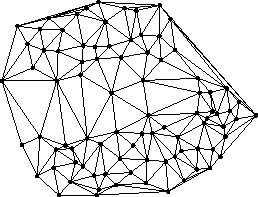
\includegraphics[width=\textwidth]{delaunay-alpha-a}
      \subcaption{Delaunay Triangulation einer beliebigen Punktmenge}
      \label{fig:delaunay-alpha-a}
    \end{subfigure}
    \hfill
    \begin{subfigure}[t]{\subwidth}
      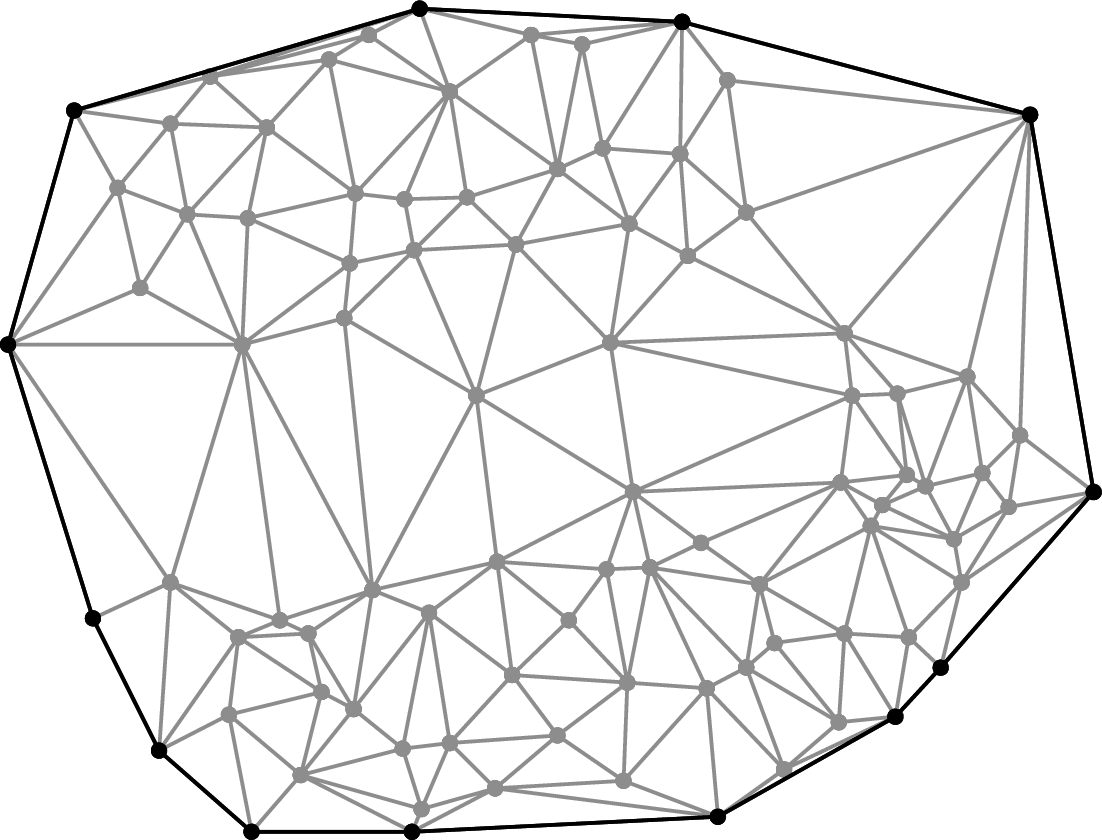
\includegraphics[width=\textwidth]{delaunay-alpha-b}
      \subcaption{Konvexe Hülle: Hülle der Triangulation}
      \label{fig:delaunay-alpha-b}
    \end{subfigure}
  }
  \vspace{2em}
  \captionsetup[subfigure]{singlelinecheck=false}{
    \def\subwidth{0.4\textwidth}
    \def\svgwidth{\textwidth}
    \begin{subfigure}[t]{\subwidth}
      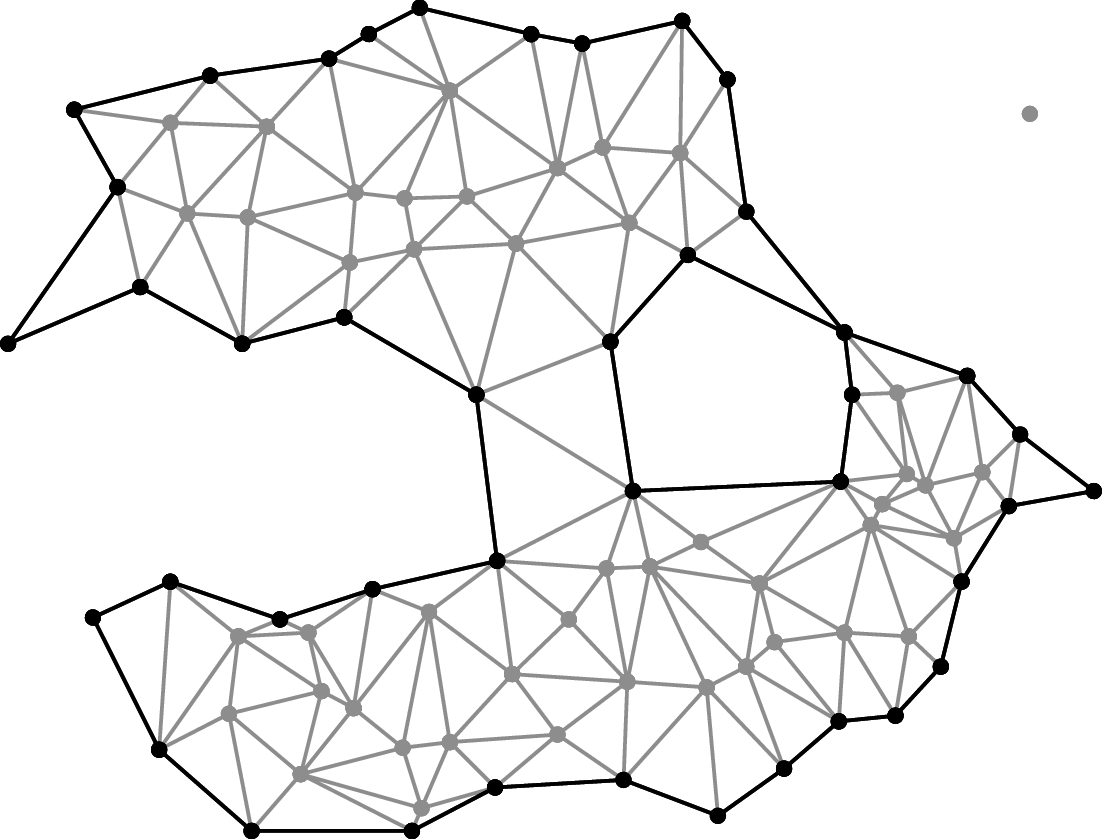
\includegraphics[width=\textwidth]{delaunay-alpha-c}
      \subcaption{Alpha-Form: Hülle nach Entfernung von Simplexen mit $r_d > \alpha$}
      \label{fig:delaunay-alpha-c}
    \end{subfigure}
    \hfill
    \begin{subfigure}[t]{\subwidth}
      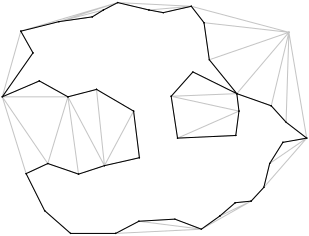
\includegraphics[width=\textwidth]{delaunay-alpha-d}
      \subcaption{Alpha-Form: Hülle nach Entfernung von Simplexen mit $r_d < \alpha$}
      \label{fig:delaunay-alpha-d}
    \end{subfigure}
  }
  \caption[Bestimmung der Oberfläche per Delaunay-Triangulation]{
    Bestimmung der Oberfläche per Delaunay-Triangulation.
    Die Alpha-Form in (d) trianguliert auch Ausreißer-Punkte, zählt sie aber ebenfalls nicht zur Hülle
  }
  \label{fig:delaunay-alpha}
\end{figure}
